\section{Estimation of Parameters}
The parameters from the wheel (mass, distance from its center to the pivoting point of the frame, inertia with respect to its center of rotation and friction) are given from a previous project.

\begin{table}[H]
	\begin{tabular}{|l|l|p{3cm}|}
		\hline %-----------------------------------------------------------------------------------
		\textbf{Parameter} &\textbf{Value} &\textbf{Units}\\
		\hline %-----------------------------------------------------------------------------------
		\si{m_w}         & \si{0,222}       &kg\\
		\hline
		%-----------------------------------------------------------------------------------
		\si{l_w}         & \si{0,093}       &m\\
		\hline %-----------------------------------------------------------------------------------
		\si{J_w}            & \si{0,601 \cdot 10^{-3}}	&\si{kg \cdot m^2}\\
		\hline  
		%-----------------------------------------------------------------------------------
		\si{B_w}         & \si{17,03 \cdot 10^{-6}}       &N \si{\cdot m \cdot s \cdot rad^{-1}}\\
		\hline
	\end{tabular}
	\caption{Parameters of the wheel}
	\label{ParametersWheel}
\end{table}

However, the rest of the parameters (\si{m_F, l_F, J_F\ and\ B_F}) must be find out. This is due to the addition of the electronics to the frame, which were not there when the tests were made.

\subsection{Mass of the Frame}
The first one to find is the mass of the frame, which can be measured weighting the setup without the base and substracting the known mass of the wheel. This gives a mass of \si{0,548\ kg}.

\subsection{Center of Mass of the Frame}
The new center of mass can be found hanging the frame from different corners and measuring he deviation angle from the vertical position in every direction. This gives a center of mass which can be seen in \figref{centerOfMassDiagram}. 
\begin{figure}[H]
	\centering
	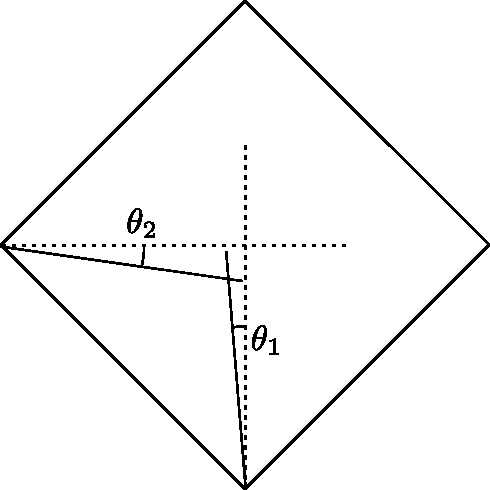
\includegraphics[scale=0.6]{figures/centerOfMassDiagram}
	\caption{Location of the center of mass, where \si{\theta_1=0.043\ rad\ and\ \theta_2=0.078\ rad}}
	\label{centerOfMassDiagram}
\end{figure}


The new point is not in the vertical line as it was assumed in the model, but this can be solved correcting the offset in the calculation of the angle inside the control loop and taking this new point as the equilibrium one. 

The new \si{l_F} can be obtained then projecting the center of mass onto the vertical line, resulting in \si{8,498\ cm}.

\subsection{Inertia and Friction of the Frame}
Finally, the new friction and inertia are estimated using a Matlab Toolbox called Senstool. \fxnote{Include SensTool manual and reference it here}

To do this estimation, the toolbox needs input and output data from a test on the real system and also a functional simulation of the model which depends on the parameters which need to be estimated. Then it tries to minimize the error between the output data and the output of the simulation, using Gauss-Newton method.

\begin{figure}[H]
	\centering
	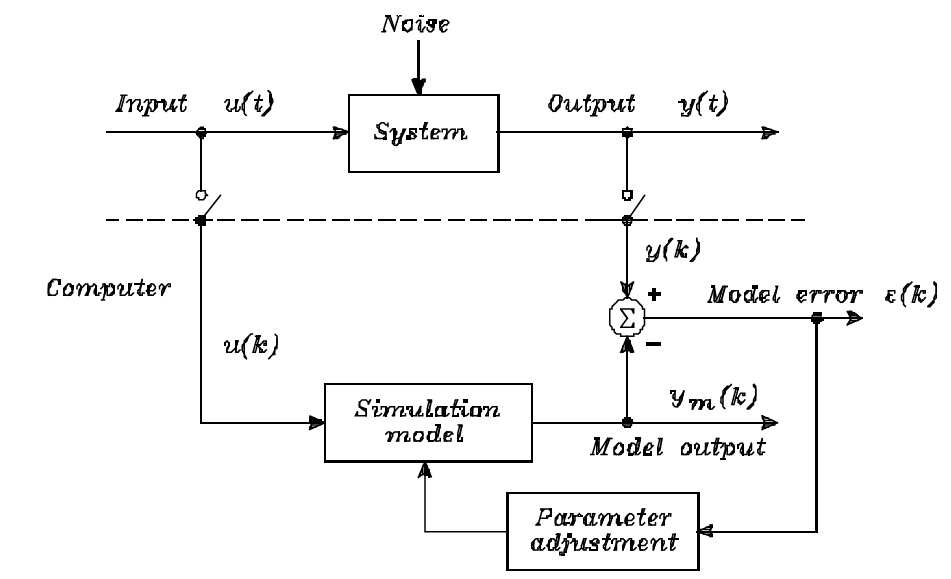
\includegraphics[scale=0.4]{figures/SensToolSchema}
	\caption{Schematic of Senstool}
	\label{SensToolSchema}
\end{figure}
The simulation of the system is given by a Simulink file, which includes the block diagram of the system without the influence of the speed of the wheel.

The data is obtained through a test described in Appendix \ref{impulseResponseAppendix}, which gives the following result:

\begin{figure}[H]
	\centering
	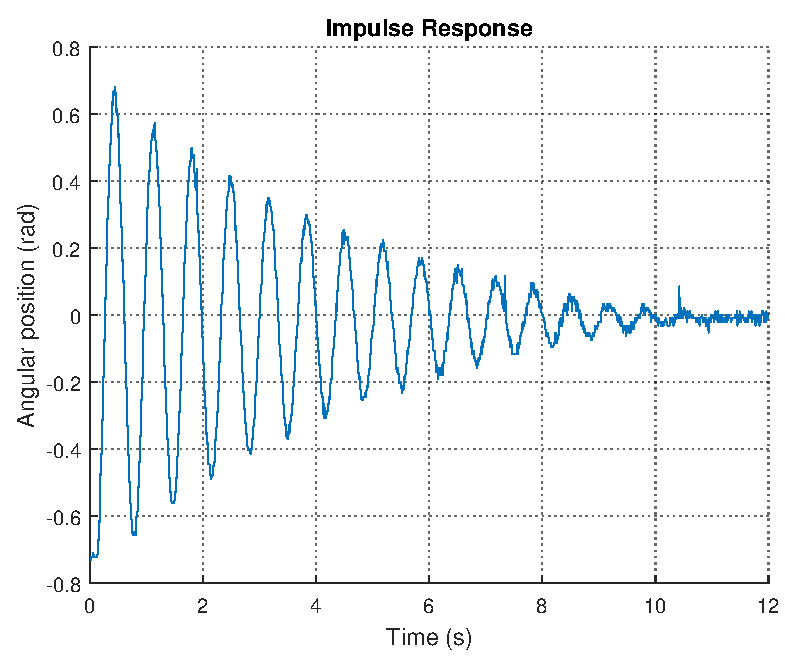
\includegraphics[scale=0.6]{figures/ImpRad}
	\caption{Angular position of the Cubli for the initial condition test}
	\label{cubliInitCondTest}
\end{figure}

As the operating angle goes from \si{-0,15\ to\ 0,15\ rad}, the behavior at this range will be better if the fit is done between this operating points.

The result of this fit is seen in \figref{SenseToolParameterEstimation}, where the final estimated parameters are \si{J_F=2,8 \cdot 10^{-3}\ kg \cdot m^2\ and\ B_F=5,2 \cdot 10^{-3}\ m \cdot s \cdot rad^{-1}}.

\begin{figure}[H]
	\centering
	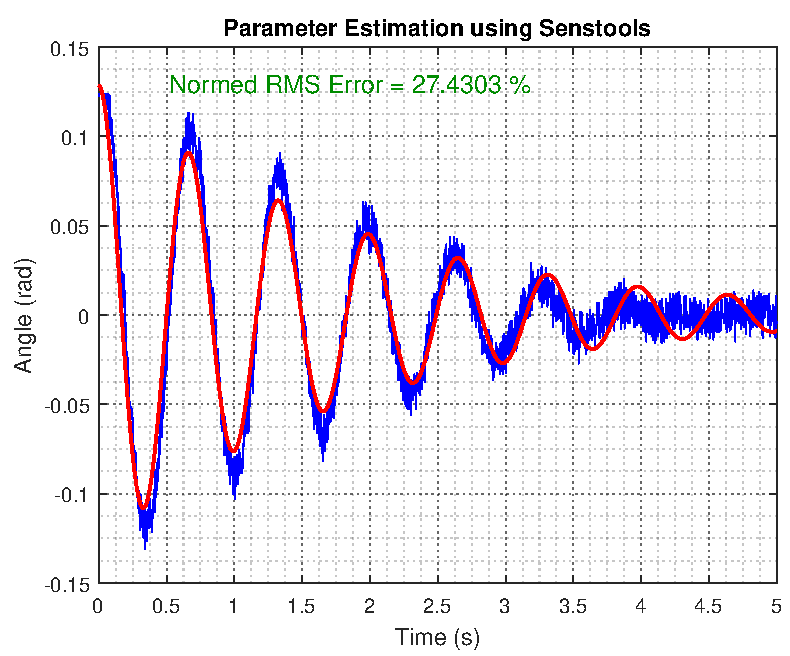
\includegraphics[scale=0.6]{figures/SenseToolParameterEstimation}
	\caption{Data from the test (red) and final fit with the new parameters (blue)}
	\label{SenseToolParameterEstimation}
\end{figure}

\subsection{Final Parameters}
The final parameters of the system can be seen in \ref{ParametersSystem}
\begin{table}[H]
	\begin{tabular}{|l|l|p{3cm}|}
		\hline %-----------------------------------------------------------------------------------
		\textbf{Parameter} &\textbf{Value} &\textbf{Units}\\
		\hline %-----------------------------------------------------------------------------------
		\si{m_w}         & \si{0,222}       &kg\\
		\hline
		%-----------------------------------------------------------------------------------
		\si{l_w}         & \si{0,096}       &m\\
		\hline %-----------------------------------------------------------------------------------
		\si{J_w}            & \si{0,601 \cdot 10^{-3}}	&\si{kg \cdot m^2}\\
		\hline  
		%-----------------------------------------------------------------------------------
		\si{B_w}         & \si{17,03 \cdot 10^{-6}}       &N \si{\cdot m \cdot s \cdot rad^{-1}}\\
		\hline
		%-----------------------------------------------------------------------------------
		\si{m_F}         & \si{0,548}       &kg\\
		\hline
		%-----------------------------------------------------------------------------------
		\si{l_w}         & \si{0,08498}       &m\\
		\hline %-----------------------------------------------------------------------------------
		\si{J_F}            & \si{2,8 \cdot 10^{-3}}	&\si{kg \cdot m^2}\\
		\hline %-----------------------------------------------------------------------------------
		\si{B_F}         & \si{5,2 \cdot 10^{-3}}       &N \si{\cdot m \cdot s \cdot rad^{-1}}\\
		\hline
	\end{tabular}
	\caption{Parameters of the whole system}
	\label{ParametersSystem}
\end{table}
